\documentclass[]{rptuseminar}

% Specify that the source file has UTF8 encoding
\usepackage[utf8]{inputenc}
% Set up the document font; font encoding (here T1) has to fit the used font.
\usepackage[T1]{fontenc}
\usepackage{lmodern}

% Load language spec
\usepackage[american]{babel}
% German article --> ngerman (n for »neue deutsche Rechtschreibung«)
% British English --> english

% For bibliography and \cite
\usepackage{cite}

% AMS extensions for math typesetting
\usepackage[intlimits]{mathtools}
\usepackage{amssymb}
% ... there are many more ...
\usepackage{bbold}
\usepackage{bussproofs}
\usepackage{wrapfig}
\usepackage{color}
\usepackage{transparent}
\definecolor{candyapplered}{rgb}{1.0, 0.03, 0.0}

% Load \todo command for notes
\usepackage{todonotes}
% Sebastian's favorite command for large inline todonotes
% Caveat: does not work well with \listoftodos
\newcommand\todoin[2][]{\todo[inline, caption={2do}, #1]{
		\begin{minipage}{\linewidth-1em}\noindent\relax#2\end{minipage}}}

% Load \includegraphics command for including pictures (pdf or png highly recommended)
\usepackage{graphicx}

% Typeset source/pseudo code
\usepackage{listings}

% Load TikZ library for creating graphics
% Using the PGF/TikZ manual and/or tex.stackexchange.com is highly adviced.
\usepackage{tikz}
% Load tikz libraries needed below (see the manual for a full list)
\usetikzlibrary{automata,positioning}

% Load \url command for easier hyperlinks without special link text
\usepackage{url}

% Load support for links in pdfs
\usepackage{hyperref}

% Defines default styling for code listings
\definecolor{gray_ulisses}{gray}{0.55}
\definecolor{green_ulises}{rgb}{0.2,0.75,0}
\lstset{%
  columns=flexible,
  keepspaces=true,
  tabsize=3,
  basicstyle={\fontfamily{tx}\ttfamily\small},
  stringstyle=\color{green_ulises},
  commentstyle=\color{gray_ulisses},
  identifierstyle=\slshape{},
  keywordstyle=\bfseries,
  numberstyle=\small\color{gray_ulisses},
  numberblanklines=false,
  inputencoding={utf8},
  belowskip=-1mm,
  escapeinside={//*}{\^^M} % Allow to set labels and the like in comments
}

% Defines a custom environment for indented shell commands
\newenvironment{displayshellcommand}{%
	\begin{quote}%
	\ttfamily%
}{%
	\end{quote}%
}

%%%%%%%%%%%%%%%%%%%%%%%%%%%%%%%%%%%%%%%%%%%%%%%%%%%%%%%%%%%%%%%%%%%%%%%%%%%%%%%

\title{Mailbox Types}
\event{Seminar: Scalable Distributed Systems in Summer term 2025}
\author{Samuel Klaaßen
  \institute{RPTU Kaiserslautern-Landau, AG Software Technology: Programming Distributed Systems}}

%%%%%%%%%%%%%%%%%%%%%%%%%%%%%%%%%%%%%%%%%%%%%%%%%%%%%%%%%%%%%%%%%%%%%%%%%%%%%%%
\begin{document}
%%%%%%%%%%%%%%%%%%%%%%%%%%%%%%%%%%%%%%%%%%%%%%%%%%%%%%%%%%%%%%%%%%%%%%%%%%%%%%%

\maketitle

%%%%%%%%%%%%%%%%%%%%%%%%%%%%%%%%%%%%%%%%%%%%%%%%%%%%%%%%%%%%%%%%%%%%%%%%%%%%%%%


\begin{abstract}

With distributed systems increasing in importance and thus programming such systems being more relevant, it is expected that research is done concerning automatic proofing of important mailbox properties like mailbox conformance and deadlock-freedom. Static assertion of properties aids developers and provides fixed guarantees for the execution of such checked systems. This report aims to summarize the most important aspects of mailbox types including the Pat language and mailbox calculus. By comparing different approaches presented by different researchers, it was found that mailbox types are indeed a powerful tool requiring only few and easy type annotations which are enough to provide strong safety conditions. However, there is no tool to apply mailbox typing to real-world languages which hinders adoption by developers. Mailbox types require more research before being ready for adoption, but the theoretical foundation is solid. Further research possibilities include improving the precision of mailbox types for capturing protocols, finding a comfortable, non-intrusive way to track mailbox dependencies, and extending the currently existing solutions to support polymorphism and generics.

\end{abstract}

%%%%%%%%%%%%%%%%%%%%%%%%%%%%%%%%%%%%%%%%%%%%%%%%%%%%%%%%%%%%%%%%%%%%%%%%%%%%%%


\section{Introduction}
\label{sec:introduction}

Distributed computing has emerged as a central strategy for providing large, scalable and complex services.
To handle a large number of distributed nodes efficiently, specialized programming languages like Go, Erlang and Elixir were developed.
These languages provide first class support for processes and messages exchanged between those.

Mailboxes are a common method to implement such systems: A mailbox is a message queue read by exactly one process but to which messages can be sent from all processes.
Typically, mailboxes provide out-of-order read support.

In such systems, the sent messages must have several characteristics which must be maintained by the processes to ensure correctness: each message must be syntactically valid and also be only sent in a correct context.
The syntactic correctness of a message is given when it adheres to a specific layout of data, like a pair of integers.
A syntactically correct message has a tag to specify its kind, as usually messages of different kinds can be sent, and stores additionally exactly the information required for that kind.

A contextually correct message respects the state of the receiving actor.
An actor might want to restrict users to only send a message of a given kind a limited number of times or requires that a message of a given type is sent before another one.


A very good example is a future variable process.
That is a process for which a value is set exactly once, and which then can provide a value on request to different nodes.
Code for such a process is shown in listing \ref{lst:futureErlang}.


\begin{figure}[ht]
\begin{minipage}[c]{0.48\linewidth}
    \begin{lstlisting}
empty_future() ->
  receive
    { set, X } -> full_future(X)
  end.

full_future(X) ->
  receive
    { get, Pid } ->
      Pid ! { reply, X },
      full_future(X);
    { set, _ } ->
      erlang:error("Multiple writes")
  end.
    \end{lstlisting}
    \caption{Implementation of a future process in Erlang\cite{fowlerSpecialDeliveryProgramming2023}.}
    \label{lst:futureErlang}
\end{minipage}
\hfill
\begin{minipage}[c]{0.48\linewidth}
    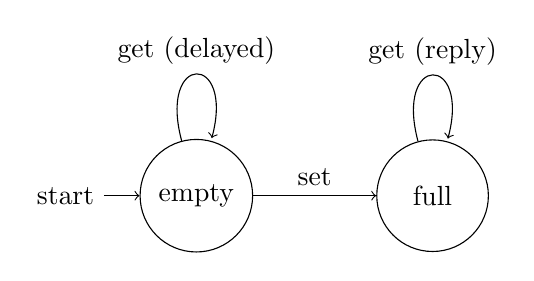
\begin{tikzpicture}[node distance=3cm,on grid,auto]
        \node[text width=1.1cm,align=center,state,initial] (s0) {empty};
        \node[text width=1.1cm,align=center,state] (s1) [right of=s0] {full};
        \path[->]
        (s0) edge node {set} (s1)
        (s0) edge [loop above] node {get (delayed)} ()
        (s1) edge [loop above] node {get (reply)} ();
    \end{tikzpicture}
    \caption{
        State automaton of a future process.
        Get requests in the empty state are not answered immediately, but their response is delayed until a value is set.
        This works because mailboxes typically provide out-of-order read access.
    }
    \label{fig:futureStateAutomaton}
\end{minipage}
\end{figure}

While syntactic checks, which guarantee that only ever correct get and set operations are sent to the future, are not overly complex and can be implemented rather easily, the restrictions expressed by the state automaton are not encoded:

For multiple set operations, an error will be generated at runtime.
The invariant that the set operation can only and must be exactly called once is not encoded.
Additionally, a process using this future will have no guarantee that the future really does send a reply.
A compiler could not check if the get operation of the consuming client erroneously precedes a set operation.
Also, the compiler does not guarantee that the future process indeed sends a reply to the get operation.

All of these issues could be resolved if we could express the automaton and the state of the process into the type system.
In the following, it is explored how mailboxes can be typed using regular expressions, so called message patterns, to achieve this.
We will determine the mailbox type $?(Set[Int] \odot \star Get[!Reply[Int]])$ for the empty future mailbox which encodes all the guarantees required for safe execution.

The research goals of this thesis are thus the following:
\begin{itemize}
    \item Present and explain mailbox typing as presented by Fowler et al.\cite{fowlerSpecialDeliveryProgramming2023}.
    \item Showcase advantages and shortcomings through case studies.
\end{itemize}


\section{Background}
\label{sec:background}

\subsection{Channel-based vs. actor-based message passing}

There are several languages with first class message passing support, generally distinguishable by two separate ideas: A channel-based system like implemented in Go makes it possible for one process to store messages in a message queue and another process can read from that queue.
This is a single connection between exactly two processes.
Those are not discussed in report.

Erlang and Elixir instead use an actor-based system where each process, called actor, is associated with a mailbox.
Each mailbox can be populated from every process by sending a message and only the owner of the mailbox can read from that queue.
The rules for reading are usually quite relaxed, with the possibility for out-of-order processing.
These mailboxes are the focus of this report.



\subsection{Mailbox validity}

Next, the properties required for a valid mailbox and its corresponding process are discussed.

\begin{description}
    \item[Mailbox conformance] That aligns closely with the syntactic correctness discussed earlier.
    A mailbox only receives messages it is designed to handle.
    There are no unexpected messages.
    While this property is not absolutely necessary for a system to be correct, it is always desirable since all unhandled messages waste resources and cannot serve a meaningful purpose.
    Sending a message which cannot be handled to a mailbox is a programming error and usually an oversight on the programmer's part.
    It is good when the type checker points out such errors.
    \item[Deadlock freedom] A deadlock refers to a situation where multiple processes wait on another but neither can continue, a cyclic dependency.
    Deadlock freedom is guaranteed when some processes eventually make progress.
    This property is necessary for the correctness of the application.
    \item[Junk freedom] All messages stored in the mailbox are eventually handled.
    That is, no message was unimportant, there was no junk.
    While this property is not always necessary for a system to be correct, it is always desired, for several reasons.
    Messages which are junk waste resources and point out that communication between several processes is not as meaningful and efficient as can be.
    When junk freedom is guaranteed, debugging is easier, and the number of edge cases are reduced. It should be noted that junk freedom will not always be guaranteed through mailbox types.
\end{description}


All three of these properties are desired and are usually fulfilled for correct systems.
Without mailbox typing, the programmer has to be attentive and has little assistance from the compiler that the properties hold.
With mailbox typing, the two former properties can be statically asserted at compile time.
If the type checker finds no error, these properties are guaranteed.


\subsection{Behavioral types}
At the heart, mailbox types are an example of behavioral types.
As behavioral types are not implemented in many languages, a small overview is given.

In many statically typed programming languages, types are only used to describe what a value is: an integer, a class or any other value.
However, that is not good enough to perform type checking that can reason about deadlock and junk freedom - those properties are dependent on the number and types of messages exchanged between processes, in short, they depend on the protocol.

Behavioral types also express the behavior of a value and can be used to specify a protocol\cite{huttelFoundationsSessionTypes2016}.

To make it more practical, imagine a queue into which a process sends an integer and then reads a boolean, put there as a response from another process, for example a query to the server if a specific id is available.
In many languages like Java or C++, it would be difficult to encode such a queue with a descriptive type, at best using two template argument like \lstinline{BidirectionalQueue<int, bool>} where each argument corresponds to the types of messages sent per direction.
However, the behavior and interplay of the two processes is not encoded in any way.
That is where behavioral types are more precise: instead of only encoding the data which could be sent, the type also directly encodes the protocol and clearly states which operations are allowed when.
In the following, we will often see a pattern like \lstinline{!int.?bool.end}.
Here, the type checker is informed that first an \lstinline{int} is sent and then a \lstinline{bool} is received.
The entire protocol is thus lifted into the type system and automatic type checking can be performed, enabling the automatic analysis of the aforementioned properties for mailbox validity.

Behavioral types can be thus used to express state: in the example, after the integer was sent, the type of the mailbox is only \lstinline{?bool.end}.
The mailbox type has changed to accommodate the change in the protocol state.
Albeit unintuitive at first, this is exactly what is required to accurately reason about the desired properties for mailboxes.


% \begin{figure}[ht]
%     \begin{lstlisting}
% // The queue is initialized with integers in the output capability
% // and bools in the input capability
% BidirectionalQueue<int, bool> queue;

% // Assuming the !int.?bool.end protocol, this operation will succeed
% // The C++ type checker will also find no error.
% queue.send(42);
% bool result = queue.receive();
%     \end{lstlisting}
% \caption{A simple send p.}
% \label{fig:behavioralTypesCpp}
% \end{figure}


\section{Topic-specific content}
\label{sec:contentSummary}

With the required background information explained, next, the typing of mailboxes is tackled.

\subsection{Mailbox types}

% Explanation of what patterns are: syntax
% they are the "goal" - annotating mailboxes with these patterns gives 
%   roughly what we want.
% how can we verify that the declarative patterns are correct?
Mailbox types are specified using a pattern and a capability, either $?$ for input or $!$ for output. Patterns are syntactically a simple recursive type, similar to regular expressions.

\begin{align*}
    E = \mathbb{0} \mid \mathbb{1} \mid \textbf{m} \mid E \oplus F \mid E \odot F \mid \star E
\end{align*}

The three recursive operators are straightforward and well-known. The atoms require more explanation: $\mathbb{0}$ encodes an error state, or, in other words, the unreliable mailbox, that is, a mailbox which has received invalid messages and cannot be used to read or send messages. That value is not strictly required for declarative typing but is helpful for theoretical analysis. $\mathbb{1}$ describes the empty pattern and \textbf{m} describes a single message.

Note that the composition $\odot$ is commutative: since mailboxes are not bound to read messages in the order they were written, ordering of messages is not important and also not considered in mailbox patterns: $E \odot F = F \odot E$.

A complete mailbox type may, for example, be $?(\textbf{set} \odot \star \textbf{get})$ which encodes a single set message followed by multiple get messages. Sometimes, the values which are transferred as payload with a message are appended in brackets to a message like so: $?(\textbf{set}[Int] \odot \star \textbf{get}[!\textbf{reply}[Int]])$. That is again the value of a mailbox for a future process. Note that the \textbf{get} messages have a mailbox as payload which the future process has to send a message to on reception. 

These mailbox types are enough to provide a declarative type system: a program could be annotated using only these types and enough information is provided to enable a type checker to assert all the properties for mailbox validity. Next, it is shown that indeed this information suffices and how that could be done.

%Generally, if a programming language supports these mailbox types and the type checker guarantees that all mailboxes requiring a message are sent a message and all messages from a mailbox are read while ensuring deadlock-freedom, 

\subsection{Mailbox calculus}

% this is solved by mailbox calculus
% explain idea 
% explain free and new
% give examples of mailbox calculus, preferrably of a future
% explain rules to check if calculus is correct
% professor likes a tree with rules: give example for future derivation

Mailbox calculus was first introduced by Padovani et al.\cite{padovaniTypeCheckingAlgorithm2018} as a mild extension of the $\pi$-calculus, previously designed by Sangiorgi et al.\cite{sangiorgiPiCalculusTheoryMobile2003}. Generally, the aim is to provide rules with premises and conclusions about processes operating on mailboxes. If the premises hold, the conclusion is correct. Some of these rules are axioms with no premises. If the rules can be composed in such a way that the implemented process is obtained, that process is typed correctly.

To provide such rules, guaranteeing correct semantics of processes, the syntax needs to be defined first. The syntax of mailbox calculus is defined in figure \ref{fig:mailboxCalcSyntax}.

\begin{figure}[ht]
    \begin{minipage}[c]{0.5\textwidth}
        \begin{align*}
    \text{Processes: } \\
    P, Q &= \text{done} \tag{termination}\\
    &\mid X[\vec{v}] \tag{invocation}\\
    &\mid G \tag{guarded process}\\
    &\mid a!\textbf{m}[\vec{v}] \tag{stored message}\\
    &\mid P | Q \tag{parallel composition}\\
    &\mid (\nu a) P \tag{mailbox restriction}
        \end{align*}
    \end{minipage}
    \hfill
    \begin{minipage}[c]{0.5\textwidth}
        \begin{align*}
    \text{Guards: } \\
    G, H &= \text{fail}\ u \tag{runtime error}\\
    &\mid \text{free}\ u.P \tag{mailbox deletion}\\
    &\mid a?\textbf{m}(\vec{v}).P \tag{selective receive}\\
    &\mid G + H \tag{guard composition}
        \end{align*}
        \vfill
    \end{minipage}
\caption{Syntactical rules for processes and guards in mailbox calculus\cite{deliguoroMailboxTypesUnordered2018}.}
\label{fig:mailboxCalcSyntax}
\end{figure}

Many of these cases are easy to understand since they are closely related to the previously discussed mailbox types. There are a few cases requiring more explanation. Recall that \textit{guards} generally refer to a branch where a single message is read and removed from a mailbox. Guards provide several clauses for each message type they handle, here represented through guard composition.

The mailbox restriction and mailbox deletion are closely coupled. The former is equivalent to creation of a new empty mailbox while the latter deletes a mailbox when it is empty. This idea is slightly different to usual actor-based implementations where mailboxes and processes are inherently linked in a 1:1 relationship. Here, mailboxes are separate and a process can own two or more mailboxes. That is why it is possible to delete them, but only if they are empty to not delete messages.

The $\text{fail }u$ guard creates a runtime error for having received an unexpected message. That is of course never executed but sometimes necessary to reason about the behavior, i.e. it is simpler to rule out failures when they are very precisely defined.

Indeed, we can observe that mailbox calculus could be a programming language. It is possible to express the future example in just a few lines:

\begin{align*}
    \text{EmptyFuture}(\textit{self}) &= \textit{self}?\textbf{set}(val).\text{FullFuture}[\textit{self}, val] \\
    \text{FullFuture}(\textit{self}, val) &= \text{free }\textit{self}.\text{done} \\
    &+ \textit{self}?\textbf{get}(sender).(sender!\textbf{reply}[val] \mid \text{FullFuture}[\textit{self}, val])\\
    &+\textit{self}?\textbf{set}.\text{fail }\textit{self}
\end{align*}

The main execution path is very similar to the Erlang implementation from listing \ref{lst:futureErlang}, although some clarifications are in order. The first case of the full future state apparently always frees the used mailbox and then terminates, but that is not the case. The free operation is only permitted if the used mailbox is empty. As long as there are messages to handle, that case cannot be executed and as soon as there are no more messages, it is the only executable case. Similarly, for the third case in the full future, it seems like the fail operation can happen when another set is performed, however, that is not the case. Processes only pass the type check if the compiler can verify that the fail operation is actually never performed.

The overarching goal with mailbox calculus is to use mailbox types to prove that a mailbox calculus implementation is correct, in our case, the implementation of the future process. Before that can be done however, deadlocks need to be analyzed.

Currently, considering the future, both of the following variants are identical, although one will work and the other will not. The typing rules will need to be extended in order to accommodate ordering and dependencies.

\begin{align*}
    \textit{future}!\textbf{set}(15).\textit{future}!\textbf{get}(\textit{self}).\textit{self}?\textbf{reply}[val] \tag{valid use of future}\\
    \textit{future}!\textbf{get}(\textit{self}).\textit{self}?\textbf{reply}[val].\textit{future}!\textbf{set}(15) \tag{invalid use of future}
\end{align*}


\subsubsection{Dependency graph} The solution to this is a dependency graph. Its main task is to encode which mailbox is dependent on which other mailbox. When cycles are created, deadlock freedom cannot be guaranteed and the program is ill-typed. Two conflicting dependencies are generated in the second case since first, the mailbox $\textit{self}$ is sent to $\textit{future}$, generating a dependency there. the conflicting dependency is generated in the guard on $\textit{self}$ because it uses the $\textit{future}$ mailbox in its clause. As we will shortly see, this conflict is accurately identified in the typing rules.


\subsubsection{Typing rules}
For reasons of space, it is impossible to repeat all required definitions used by the typing rules nor is it feasible to present all typing rules in detail. However, looking at a few of the rules and observing an interplay of many different rules to prove the correctness of the future examples is a worthwhile endeavor.

\begin{prooftree}
    \AxiomC{$\Gamma \vdash P :: \varphi$}
    \RightLabel{\scriptsize\textsc{[t-free]}}
    \UnaryInfC{$u : ? \mathbb{1}, \Gamma \vdash \text{free } u.P$}
\end{prooftree}

This rule is used to constrain and develop an operation to free a mailbox. Left of $\vdash$, the so called \textit{type environment} is written. It assigns a type to each free variable on the right side of $\vdash$. Some rules are followed by a $:: \varphi$ which is the dependency graph by the expression.

To correctly read the rule, start at the top: assuming under a given type environment, $P$ is valid and produces a dependency graph $\varphi$, the expression $\text{free }u.P$ is also valid, but with an additional type where $u$ has type $?\mathbb{1}$. This is a logical result since it encodes that only exactly the empty mailbox can be freed.

For a better understanding, the rule for production of new mailboxes is analyzed.

\begin{prooftree}
    \AxiomC{$\Gamma, a : ?\mathbb{1} \vdash P :: \varphi$}
    \RightLabel{\scriptsize\textsc{[t-new]}}
    \UnaryInfC{$\Gamma \vdash (\nu a) P :: (\nu a)\varphi$}
\end{prooftree}

Here, it is observable that the free variable $a$ bound in the type environment which appears somewhere in $P$ is bound to a value using the mailbox restriction syntax defined in figure \ref{fig:mailboxCalcSyntax}. $a$ is then dropped from the type environment. The dependency graph is also modified, but that operation will not be covered.

It is never explicitly mentioned what happens when the dependency graph determines a cyclic dependency, but it is safe to assume that the proof found a deadlock and can thus be aborted.

Now, using additional rules, it will be interesting to see the future process being verified by building of such a tree. For reasons of space, abbreviations are necessary.
\begin{align*}
    \rho &= ?\textbf{reply}[Int]
    &\delta = !\textbf{get}[\rho]\hspace{2cm}
    \tau &= !\textbf{put}[Int] 
    &F = \tau \cdot \delta^*
\end{align*}

%TODO
\newsavebox{\futureprooftree}
% \savebox{\futureprooftree}{
\resizebox{0.85\textwidth}{!}{\begin{minipage}{\textwidth}
    
    \begin{prooftree}
        % leftest msg f!get(c)
        \AxiomC{}
        \RightLabel{\scriptsize\textsc{[t-msg]}}
        \UnaryInfC{$f: \delta, c: \rho \vdash f!\textbf{get}[c] :: \{ f, c\}$}

        % %f!put[3]
        \AxiomC{}
        \RightLabel{\scriptsize\textsc{[t-msg]}}
        \UnaryInfC{$f: \tau, \vdash f!\textbf{put}[3] :: \emptyset$}

        \RightLabel{\scriptsize\textsc{[t-par]}}
        \BinaryInfC{$f: \delta \cdot \tau, c: \rho, \vdash f!\textbf{get}[c] \mid f!\textbf{put}[3] :: \{ f, c\}$}

        
        \AxiomC{}
        \RightLabel{\scriptsize\textsc{[t-done]}}
        \UnaryInfC{$\emptyset \vdash \text{done} :: \emptyset$}
        \RightLabel{\scriptsize\textsc{[t-free]}}
        \UnaryInfC{$c: ?\mathbb{1} \vdash \text{free }c.\text{done}$}
        \RightLabel{\scriptsize\textsc{[t-guard]}}
        \UnaryInfC{$c: ?\mathbb{1} \vdash \text{free }c.\text{done} :: \emptyset$}
        \RightLabel{\scriptsize\textsc{[t-in]}}
        \UnaryInfC{$c: \rho \vdash c?\textbf{reply}(x).\text{free }c.\text{done}$}
        \RightLabel{\scriptsize\textsc{[t-guard]}}
        \UnaryInfC{$c: \rho \vdash c?\textbf{reply}(x).\text{free }c.\text{done} :: \emptyset$}


        \RightLabel{\scriptsize\textsc{[t-par]}}
        \BinaryInfC{$f: \delta \cdot \tau, c: \rho, \vdash f!\textbf{get}[c] \mid f!\textbf{put}[3] \mid c?\textbf{reply}(x).\text{free }c.\text{done} :: \{ f, c\}$}

        \RightLabel{\scriptsize\textsc{[t-sub]}}
        \UnaryInfC{$f: \delta \cdot \tau^*, c: \rho, \vdash !\textbf{get}[c] \mid f!\textbf{put}[3] \mid c?\textbf{reply}(x).\text{free }c.\text{done} :: \{ f, c\}$}

        \RightLabel{\scriptsize\textsc{[t-new]}}
        \UnaryInfC{$f: !F, \vdash (\nu c)(!\textbf{get}[c] \mid f!\textbf{put}[3] \mid c?\textbf{reply}(x).\text{free }c.\text{done}) :: (\nu c)\{ f, c\}$}
    \end{prooftree}

    \vspace{0.8cm}
\end{minipage}
}


As can be seen, proof trees can be messy even for small examples. Nonetheless, the proof can clearly be seen in the last line. Given process $f$ has the future type $!F$, the following expression is well-typed with mailbox conformance and deadlock-freedom. Padovani et al.\cite{deliguoroMailboxTypesUnordered2018} present also the counterexample: if the put operation follows the reply, the process is ill-typed and a deadlock is detected.




\subsubsection{Summary}

It was proven by Padovani et al.\cite{deliguoroMailboxTypesUnordered2018} that a well-typed process is mailbox conformant and deadlock-free, more precisely, if a conclusion of the kind $\emptyset \vdash P :: \varphi$ is reached, then the defined process $P$ is mailbox conformant and deadlock-free. The third property of junk freeness is also guaranteed in some cases, most importantly for all process with a finite number of invocations. Then junk freedom can even be guaranteed for some recursive processes, provided they are only repeated finitely many times.

Overall, this typing procedure gave a very strong result with fairly little complexity. The proposal by Padovani et al.\cite{deliguoroMailboxTypesUnordered2018} has proven that mailbox types as described above are sufficient to guarantee the most important properties for mailbox types, and although a rule set was provided which can prove the correctness of given declarations, the algorithmic construction of such a proof tree was not considered. To create a type checker, that is an unavoidable obstacle. 


\subsection{Applying Mailbox calculus on Pat}

% explain the programming language pat
% pretty close direct translation of mailbox calculus
% explain additional problems: aliasing
% solution: quasi-linearity and usage annotations


Fowler et al.\cite{fowlerSpecialDeliveryProgramming2023} build upon mailbox calculus by integrating the proposed mailbox types into a custom programming language called Pat and provide a type checker\cite{fowlerPatCheckerGithub2025} for that language. 



An example implementation of the future process in Pat can be seen in listing \ref{lst:futurePat}. While the adaption from mailbox calculus to a separate programming language seems simple, there are two large issues not yet discussed. The first is aliasing, that is, how to handle it when mailboxes are renamed, and the second is that a proof tree needs to be constructed automatically.

\begin{wrapfigure}{r}{0.5\textwidth}
\vspace{-20pt} % Adjust as needed
\begin{lstlisting}
interface Future { Set(Int), Get(User!) }
interface User   { Reply(Int) }

def emptyFuture(self: Future?): Unit {
  guard self : Set . Get* {
    receive Set(x) from self ->
      fullFuture(self, x)
  }
}

def fullFuture(self: Future?, value: Int)
  : Unit
  {
  guard self : Get* {
    free -> ()
    receive Get(user) from self ->
      user ! Reply(value);
      fullFuture(self, value)
  }
}
\end{lstlisting}
\caption{An implementation of a future process in Pat.\cite{fowlerPatCheckerGithub2025}}
\label{lst:futurePat}
\vspace{-20pt} % Adjust as needed


\end{wrapfigure}

\subsubsection{Aliasing}

Variable names are an important part of programming languages and thus, programming languages provide a method to bind names to values. In Pat, this is implemented by providing a \lstinline|let name = value in <...>| expression, however, mailboxes can also be aliased using this method, resulting in potential use-after-free errors. A dependency graph was used above to circumvent those errors by creating a connection between mailbox names. In Pat however, the generation of mailboxes is not directly expressed in static process information as in mailbox calculus and the compiler cannot accurately reason about mailbox identities.

\begin{wrapfigure}{l}{0.4\textwidth}
\begin{lstlisting}[escapechar=/]
interface It { Msg(Int) }

def useAfterFree(x: It?): Unit {
    guard x : Msg* {
        receive Msg(val) from y ->
            (); useAfterFree(y)
        free -> /\transparent{0.3}\colorbox{candyapplered}{\transparent{1.0}x ! Msg(4)}/
    }
}

let mb = new[It] in
mb ! Msg(3);
useAfterFree(mb)
\end{lstlisting}
\caption{A use-after-free error. The highlighted operation is not permitted since the mailbox \lstinline|x| has been freed.\cite{fowlerSpecialDeliveryProgramming2023}}
\label{lst:patUseAfterFree}
\vspace{-00pt}
\end{wrapfigure}

To see, how mailboxes can be created and how incorrect use can result in errors, a simple example program can be seen in listing \ref{lst:patUseAfterFree}. This is just one example, characterized by Fowler et al. as using the old name. A simple check that the mailbox being guarded upon is not used in the free guard is insufficient as it could also be aliased using a \lstinline|let|-binding or the guard could be performed in a separate evaluation context.

With the dependency graph being not usable to check for correctness in these scenarios, an alternative solution was proposed: quasi-linear typing. 

Mailboxes are annotated by the compiler, in addition to their pattern and capability, with a usage: either a \textit{returnable} or a \textit{second-class} reference. Here, the returnable references are stronger and provide more capabilities although they also have more limitations. The main idea is that only one returnable reference exists for a mailbox and when that is guaranteed, guard operations can be limited to only be allowed for returnable references. A check for use-after-free errors is then easy to perform. Returnable references can only be consumed once, for example, after a returnable reference was assigned to a new name, that value can no longer be used.

There still exists a loophole: when sending a mailbox to another process via a message argument, the original process keeps its returnable reference since it was not consumed and the new process would also have access to a returnable reference. That is explicitly forbidden by treating all received mailboxes as second-class.

\subsubsection{Type checking}

To type check a declarative Pat program, a tree of the rules building the given program must be synthesized. The most complete approach for this problem is described by Padovani\cite{padovaniTypeCheckingAlgorithm2018}. Instead of trying to build a tree from the rules that were explained for mailbox calculus, a different set of rules is used which are proven to be equivalent. The main idea of building such a tree backwards is that joins of type environments is a simple operation, but splitting a type environment, which would be required when starting with a large expression and branching into smaller parts, is more difficult.

Padovani describes three main ideas.
\begin{enumerate}
    \item The tree is not built with the goal of a given type environment, but the rules generate a valid type environment.
    \item If at a given point in time the information is not enough for now to determine a type, a type variable is instead used.
    \item When subtyping cannot be verified when encountering them, these relations are instead in encoded in type constraints. These type constraints will have to be solved in order for the type check to succeed.
\end{enumerate}


For Pat, these ideas are extended with bidirectional typing where instead of type constraints, inclusion constraints are used. Inclusion constraints operate on pattern variables. These do not exist in the declarative type system and are a placeholder for a part of pattern. These inclusion constraints have the form $\gamma \lessdot \delta$ where $\gamma$ has to be included in $\beta$. To give an example of when such a constraint can be generated, when calculating the joint type of two mailboxes with the types $!\textbf{m}$ and $?(\textbf{m} \odot \textbf{n})$ is $?\alpha$ where $\alpha$ is constrained by $(\textbf{m} \odot \alpha) \lessdot (\textbf{m} \odot \textbf{n})$. The solution in that case can be $\alpha = \textbf{n}$. 

To give an example of such a type checking rule working from bottom up, the \lstinline|guard| rule is showcased:

\begin{prooftree}
    \AxiomC{$\{E\} \vec{G} \Leftarrow \tau \blacktriangleright \Psi; \Phi_1; F$}
    \AxiomC{$V \Leftarrow ?F^\bullet \blacktriangleright \Theta';\Phi_2$}
    \AxiomC{$\Psi + \Theta' \blacktriangleright \Theta ; \Phi_3$}
    \RightLabel{\scriptsize\textsc{[tc-guard]}}
    \TrinaryInfC{$\textbf{guard } V : E \{ \vec{G} \} \Leftarrow \tau \blacktriangleright \Theta; \Psi_1 \cup \Psi_2 \cup \Psi_3 \cup \{ E \lessdot F\}$}
\end{prooftree}

This rule has three premises. First, the return type of the guard expression has to match. This first premise also sets the pattern $F$ which is consumed by the guard expression. Second, the value being guarded upon has to match the specified pattern. The third premise is used to compute an environment by combining the environments of the first two premises. The result is a well-typed guard expression with a combined environment as well as several inclusion constraints carried over and added to them a constraint that the pattern handled in this guard expression is contained in the pattern provided by the value $V$.

As one can see, the rules are quite extensive. They are all covered and explained by Fowler et al.\cite{fowlerSpecialDeliveryProgramming2023}.

These rules are designed to be easily combinable and the only thing missing is the solving of constraints. This is done by rewriting the set of constraints into a system of closed inclusion constraints. Those can be translated into Presburger formulae and Z3 is used to check whether each constraint holds.


\subsection{Theoretical limits}
% here, i would like an example of a correct program which is flagged to be incorrect by the type checker.
% i would say: patterns are regex, so equivalent to deterministic automatons: if the actor is determinstic from the pov of the type checker, it can be checked.
% obviously, there are cases only coverable by dependable types, but that is not really interesting
% are there are actual intersting use-cases?
% i guess the usage annotations could be sub-optimal?
% otherwise: quite solid.

The theoretical limits of the Pat language are quite high: mailbox types are commutative regular expressions, so they are able to encode a lot of protocol state machines. For example, the context-free language $\{ !a^n !b^n \}$ becomes encodable since it can be rewritten using commutativity to $\{ !(a \odot b)^n \}$. However, this can also be a disadvantage: commutative regular expressions are always fully commutative, but protocol specifications are sometimes not. Imagine a protocol where a user provides login credentials and then accesses private data in a setup like $!\textbf{Login}(id).!\textbf{Access}()*$. Pat's full commutativity cannot encode the ordering of the messages although the protocol requires it. The implementation for this process can be seen in listing \ref{lst:patCommutativity}.

Here, an access operation could be processed out-of-order which then is denied. If the login message had been handled first, the access would have succeeded. Pat provides better ways to handle this method, but the problem remains the same: To express clear sequentiality, mailbox patterns are insufficient. Pat's type checker still provides too few restrictions for this case. Note that the violating access guard in the logged out state is not required and the Pat program checks successfully without it alleviating the problem.

\begin{wrapfigure}{r}{0.5\textwidth}
\begin{lstlisting}
interface It { Login(Int), Access(Bool) }

def loggedOut(x: It?): Unit {
    guard x : Login . Access* {
        receive Login(int) from y ->
            loggedIn(y)
        receive Access(b) from y ->
            (); #access is denied
            loggedOut(y)
    }
}

def loggedIn(x: It?): Unit {
    guard x : Access* {
        receive Access(b) from y ->
            (); #access is allowed
            loggedIn(y)
        free -> ()
    }
}
\end{lstlisting}
\caption{A process where Pat cannot enforce order of messages. The programmer cannot describe sequentiality using a simple mailbox pattern.}
\label{lst:patCommutativity}
\end{wrapfigure}

By encoding a clear dependency between the login and the accesses only after a login, Pat still manages to guarantee sequential access.

\begin{lstlisting}
interface User { Login(Int, Access?) }
interface Access { File(Int) }
\end{lstlisting}
\vspace{0.4cm}

These message interfaces provide a clear dependency enforceable by Pat.

However, this required a change in the protocol and the signature of the messages is different. This is designed to show that mailbox types, while very powerful, are not exactly equivalent every possible signature of a process. 

The inherent problem is that mailboxes are indeed agnostic of order and it makes sense for mailboxes types to follow suit and be fully commutative. However, as soon as a \lstinline|guard| is executed, the relaxation of ordering for messages is applied to the ordering of processing of messages and that can be bad. Maybe it makes sense to extend mailbox types to allow sequential messages and thus guarantee sequential processing.

Other limitations are few: obviously, cases where a specific number of messages are expected, but the exact number is only known at runtime cannot be encoded. Such behavior would require dependable typing which is not a limitation of Pat, but rather something it does not even try to achieve.


%TODO savina benchmark

\section{Discussion}
\label{sec:discussion}

Mailbox typing can successfully be deployed for many protocols guaranteeing important safety properties like mailbox conformance and deadlock-freedom. The rules and typing patterns are quite expressive and allow for a lot of freedom. 

The future example was expressed in multiple different versions to ensure comparability and it one can observe that the mailbox types did not hinder syntactical simplicty while providing safety guarantees. In fact, that the future process has become simpler since less invariants are implicit.

It is impossible to give a verdict on how good these ideas are in practice since there is not practical support for any of these ideas. The implemented type checkers for mailbox calculus by Padovani et al.\cite{padovaniBoystrangeMCC2024} as well as the one for Pat\cite{fowlerPatCheckerGithub2025} only provide prototypes for esoteric languages. 

Some ideas for future research would be the following:
\begin{enumerate}
    \item Find a closer relationship between the requirements for processes used in practice and identify types for their mailboxes. Processes are more complex than DFAs but usually not as complex as context-sensitive languages. Studying these state automatons might yield more insight into a theoretically solid foundation for the requirements of mailbox types.
    \item Implement tooling to aid development. Fowler et al.\cite{fowlerSpecialDeliveryProgramming2023} that their work is still ongoing with both, a type checker for mainstream actor languages as well as a transpiler from languages like Pat to common and reliable languages like Erlang, similar to Typescript. Any of these projects would enable first practical tests and would definitely provide valuable insights for extracting the requirements for mailbox typings. Additionally, migration to this new type system is an open issue and might be very difficult and complex for large systems.
    \item The usage annotations in Pat are very odd to work with and the dependency graph for mailbox calculus being much less intrusive from the point of view of the developer. Probably, a more permissible solution exists for these problems. If not, a proof would be in order.
    \item Then, the question for necessity is open. Obviously, large and very complex systems run quite well, providing these properties without an additional type checker. Although only of minor interest to researchers, businesses would adopt these mailbox type much quicker if undisputable numbers would prove the benefit of these systems. This could maybe also give an explanation why, although these types have a strong theoretical foundation and provide important safety guarantees, only little research is happening for this field of research.
    \item Several features of common programming languages are not implemented in Pat. Lists are an obvious example, but not really interesting as their implementation seems rather straightforward, especially if kept immutable. Polymorphism and generics on the other hand are not trivial to implement. Research on these topics would benefit future work when applying these type systems on languages already supporting those features.
\end{enumerate}



\section{Conclusion}
\label{sec:conclusions}

In this report, the approach to type mailboxes in actor-based systems according to Padovani et al.\cite{deliguoroMailboxTypesUnordered2018} was presented and shortly explained. Mailbox types were syntactically and semantically explained and a type rule system to prove mailbox conformance, deadlock-freedom and junk freedom was discussed. The follow-up implementation by Fowler et al.\cite{fowlerSpecialDeliveryProgramming2023} was also discussed and showcased. Instead of a dependency graph, it used quasi-linear typing to handle aliasing and dependency issues. Additionally, an implementation was given how a proof tree can be built by an automated type checker.

The key conclusions to draw is that this methodology is highly capable: with only little and very intuitive type annotations, runtime errors can be very elegantly prevented.
% theoretical limitations
Theoretical limitations are few and can also be tackled in the future.
The most pressing issues for adoption are practical support: currently, no language, besides Pat, provides support for these types. Both, for research and users, developer tools allowing quick adoption would be beneficial.




%%%%%%%%%%%%%%%%%%%%%%%%%%%%%%%%%%%%%%%%%%%%%%%%%%%%%%%%%%%%%%%%%%%%%%%%%%%%%%%
\newpage
\nocite{*}
\bibliographystyle{eptcs}
\bibliography{references}

%%%%%%%%%%%%%%%%%%%%%%%%%%%%%%%%%%%%%%%%%%%%%%%%%%%%%%%%%%%%%%%%%%%%%%%%%%%%%%%
\end{document}
%%%%%%%%%%%%%%%%%%%%%%%%%%%%%%%%%%%%%%%%%%%%%%%%%%%%%%%%%%%%%%%%%%%%%%%%%%%%%%%